\documentclass[a4paper, 12pt]{article}

\usepackage[T2A]{fontenc}
\usepackage[utf8]{inputenc}
\usepackage[english, russian]{babel}
\usepackage{amsmath}
\usepackage{graphicx}
\usepackage{subcaption}
\usepackage{float}
\usepackage{tabularx}
\usepackage{amsmath,booktabs}
\usepackage{array}
\righthyphenmin=2
\usepackage[left=20mm, top=20mm, right=20mm, bottom=20mm]{geometry} % настройки полей документа
\usepackage{caption}
\usepackage{makecell}

% Paragraph indent
\usepackage{indentfirst}
\setlength{\parindent}{15mm}

%%%%%%%TITUL%%%%%%%
\newcommand\tline[2]{$\underset{\text{#1}}{\text{\underline{\hspace{#2}}}}$}

%%%%%%%%%%%%CAPTION%%%%%%%
\usepackage{threeparttable}
%Change label separator
\usepackage{caption}
\captionsetup[table]{labelformat=simple, labelsep = endash, justification = raggedright, singlelinecheck = off, width = 0.75\textwidth}
\captionsetup[figure]{labelformat=simple, labelsep = endash, name = Рисунок}
%%%%%%%TABLE%%%%
\renewcommand{\arraystretch}{1.3}
\renewcommand{\tabcolsep}{0.7cm}

%%%%%%%%%%%%%%%%%%%%%%%%%%%%%%%%%%
\begin{document} 
	
		\begin{titlepage}
		\centering
		{\fontsize{12pt}{5cm}\selectfont \bfseries Министерство образования и науки Российской Федерации} \\ \vspace{0.5cm}
		{\fontsize{7pt}{5cm}\selectfont ФЕДЕРАЛЬНОЕ ГОСУДАРСТВЕННОЕ АВТОНОМНОЕ ОБРАЗОВАТЕЛЬНОЕ УЧРЕЖДЕНИЕ ВЫСШЕГО ПРОФЕССИОНАЛЬНОГО ОБРАЗОВАНИЯ} \\ 
		\vspace{1cm}
		{\fontsize{12pt}{5cm}\selectfont \bfseries САНКТ-ПЕТЕРБУРГСКИЙ УНИВЕРСИТЕТ ИНФОРМАЦИОННЫХ ТЕХНОЛОГИЙ, МЕХАНИКИ И ОПТИКИ} \\ \vspace{1.5cm}
		
		{\fontsize{14pt}{5cm}\selectfont Кафедра \hspace{1cm} \underline{Систем Управления и Информатики}  \hspace{1cm} Группа \underline{Р3340}} \\ 
		\vspace{2cm}
		
		{\fontsize{20pt}{5cm}\selectfont \bfseries Лабораторная работа №12} \\
		{\fontsize{20pt}{5cm}\selectfont \bfseries “Анализ линейных непрерывных систем с использованием прикладного пакета matlab control system toolbox”} \\
		{\fontsize{14pt}{5cm}\selectfont Вариант - 02} \\
		\vspace{1.5cm}
		
		\flushleft
		
		{Выполнил \hspace{0.5cm} \tline{(фамилия, и.о.)}{10cm} (подпись)} \\
		\vspace{2cm}
		
		{Проверил \hspace{0.5cm} \tline{(фамилия, и.о.)}{10cm} (подпись)} \\
		\vspace{5cm}
		
		"\underline{\hspace{0.4cm}}"\hspace{0.1cm}\underline{\hspace{1.5cm}}\hspace{0.1cm}20\underline{\hspace{0.4cm}}г. \hspace{2cm} Санкт-Петербург, \hspace{2cm} 20\underline{\hspace{0.4cm}}г. \\ \vspace{1cm}
		
		Работа выполнена с оценкой \hspace{0.5cm} \underline{\hspace{10cm}} \\ 
		\vspace{1cm}
		Дата защиты "\underline{\hspace{0.4cm}}"\hspace{0.1cm}\underline{\hspace{1.5cm}}\hspace{0.1cm}20\underline{\hspace{0.4cm}}г.
		
		\end{titlepage}

\section*{Цель работы}
Исследование динамических и частотных характеристик, анализ структурных свойств и устойчивости линейных непрерывных систем с помощью прикладного пакета Matlab Control System Toolbox.\par
В качестве исследования выбраны линейные непрерывные динамические стационарные системы. Исходная модель  разомкнутой системы представлена в форме вход-выход и описывается передаточной функцией вида:\par
\begin{align}
	W(s) = \frac{b_1s + b_0}{s\cdot(a_2s^2 + a_1s + a_0)}
	\label{w}
\end{align}

\section*{Исходные данные}
Значения коэффициентов, приведенных в таблице \ref{tab:dateTab},  $a_0, a_1, a_2, b_0, b_1$ в числителе и знаменателе передаточной функции \ref{w}, выбираются произвольно, причем $a_2 \neq 0, b_1 \neq 0$.

\begin{table}[h!]
	\centering
	\begin{threeparttable}
		\caption{Коэффициенты передаточной функции}
		\begin{tabular}{|c|c|c|c|c|}
			\hline
			$a_0$	&	$a_1$	&	$a_2$	&	$b_0$	&	$b_1$\\
			\hline
			3		&	6		&	1		&	5		&	1\\
			\hline	
		\end{tabular}
		\label{tab:dateTab}
	\end{threeparttable}
\end{table}

\newpage

\begin{center}
	\section{Анализ исходной разомкнутой системы}
\end{center}\par
Исходя из выбранных нами исходных значений передаточная функция разомкнутой системы принимает вид:
\begin{align}	
	W(s) = \frac{s + 5}{s(s^2 + 6s + 3)} = \frac{s + 5}{s^3 + 6s + 3s + 1}
	\label{w_my}
\end{align}\par
Найдем нули и полюса функции аналитически и при помощи функции Matlab - pzmap графически изобразим найденные решения на рисунке \ref{pzmap}.\par

Из функции \ref{w_my}  находим нули и полюса:

\begin{equation}
	\begin{cases}
		z_1 = 5\\	
		p_1 = -5.48\\	
		p_2 = -0.25 + j0.34\\	
		p_3 = -0.25 - j0.34
	\end{cases}
\end{equation}



\begin{figure}[h!]
	\centering
	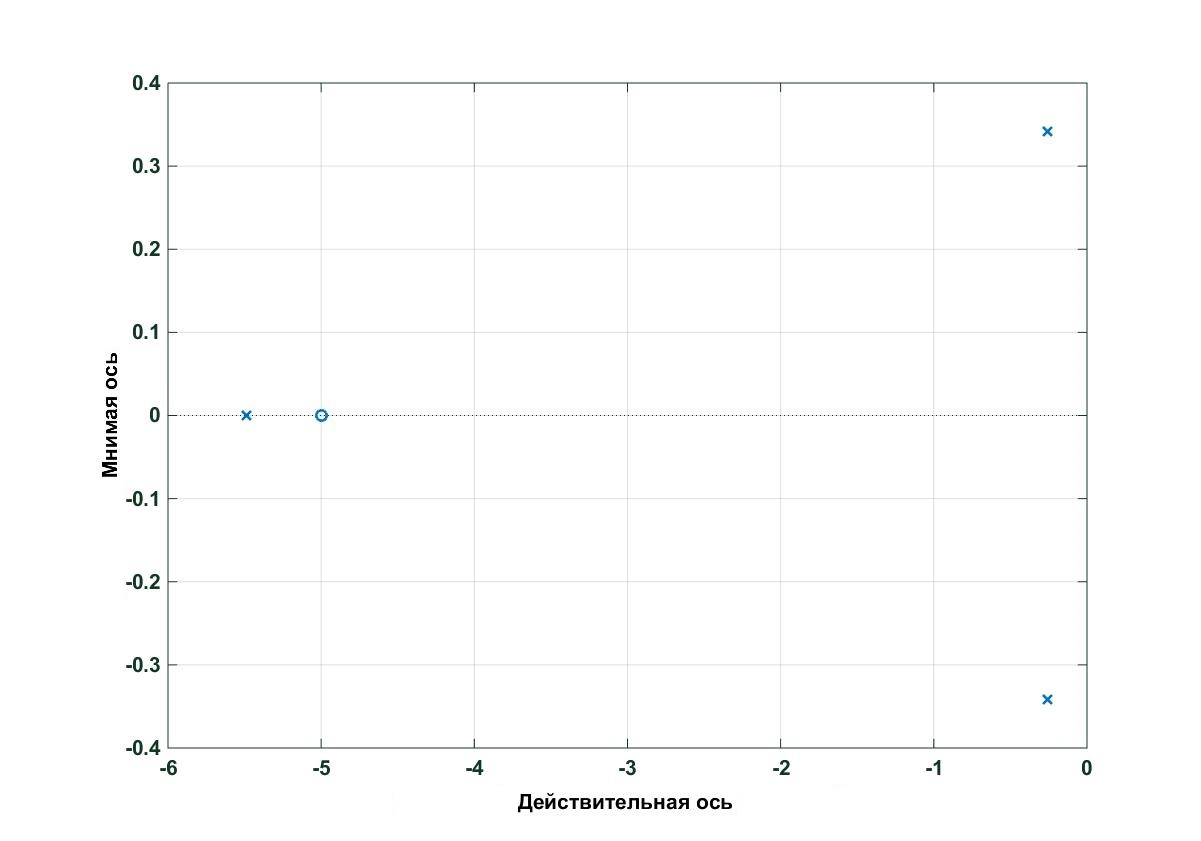
\includegraphics[width = 0.6\textheight]{data/pzmap}
	\caption{Нули и полюса разомкнутой системы}
	\label{pzmap}
\end{figure}
Далее построим логарифмические АЧХ и ФЧК с помощью команды Matlab - margin. График, полученный в результате работы функции приведен на рисунке \ref{margin}

\newpage

\begin{figure}[h!]
	\centering
	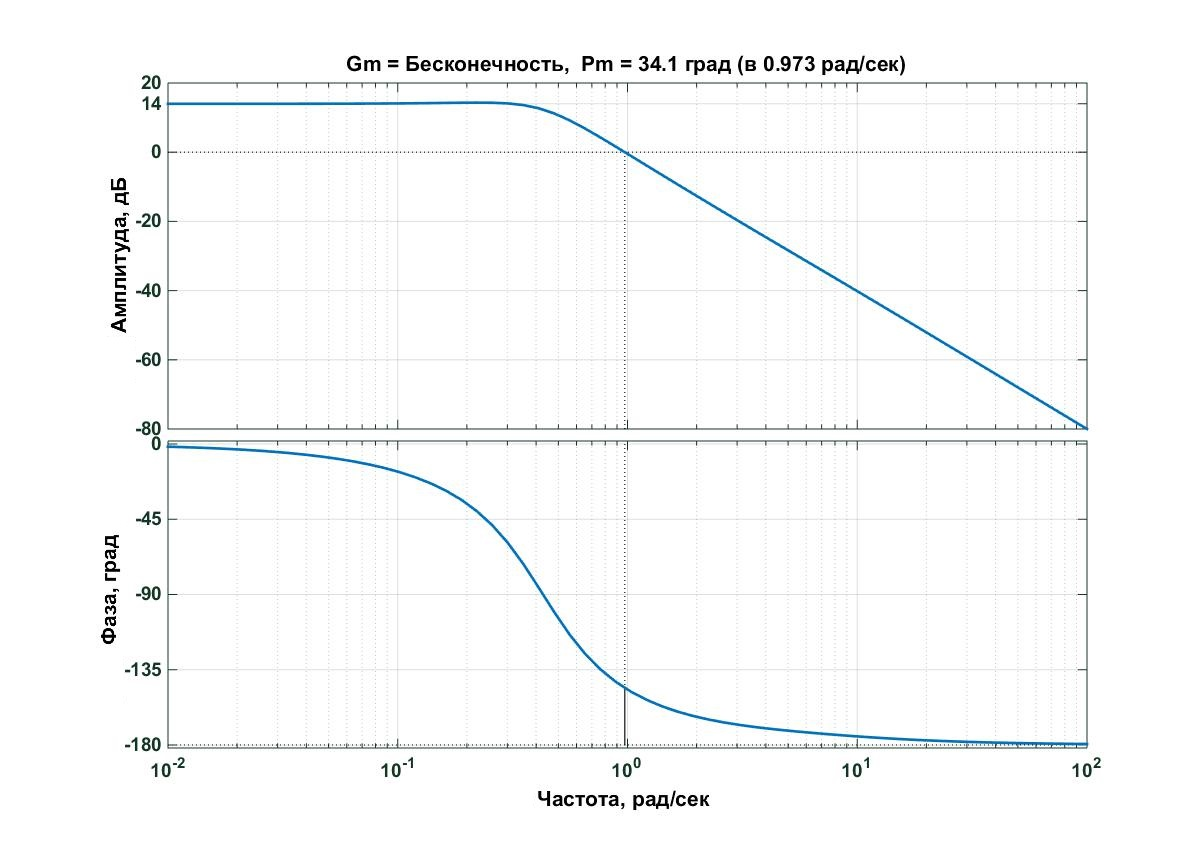
\includegraphics[width = 0.6\textheight]{data/margin}
	\caption{Логарифмические характеристики разомкнутой системы}
	\label{margin}
\end{figure}

Из рисунка \ref{margin} видно, что запас устойчивости по амплитуде - $\infty$, по фазе $34.1^{\circ}$.

\newpage

При помощи функции nyquist построим АФЧХ переходной функции \ref{w_my}. Результат работы функции приведен на  рисунке \ref{nyquist}

\begin{figure}[h!]
	\centering
	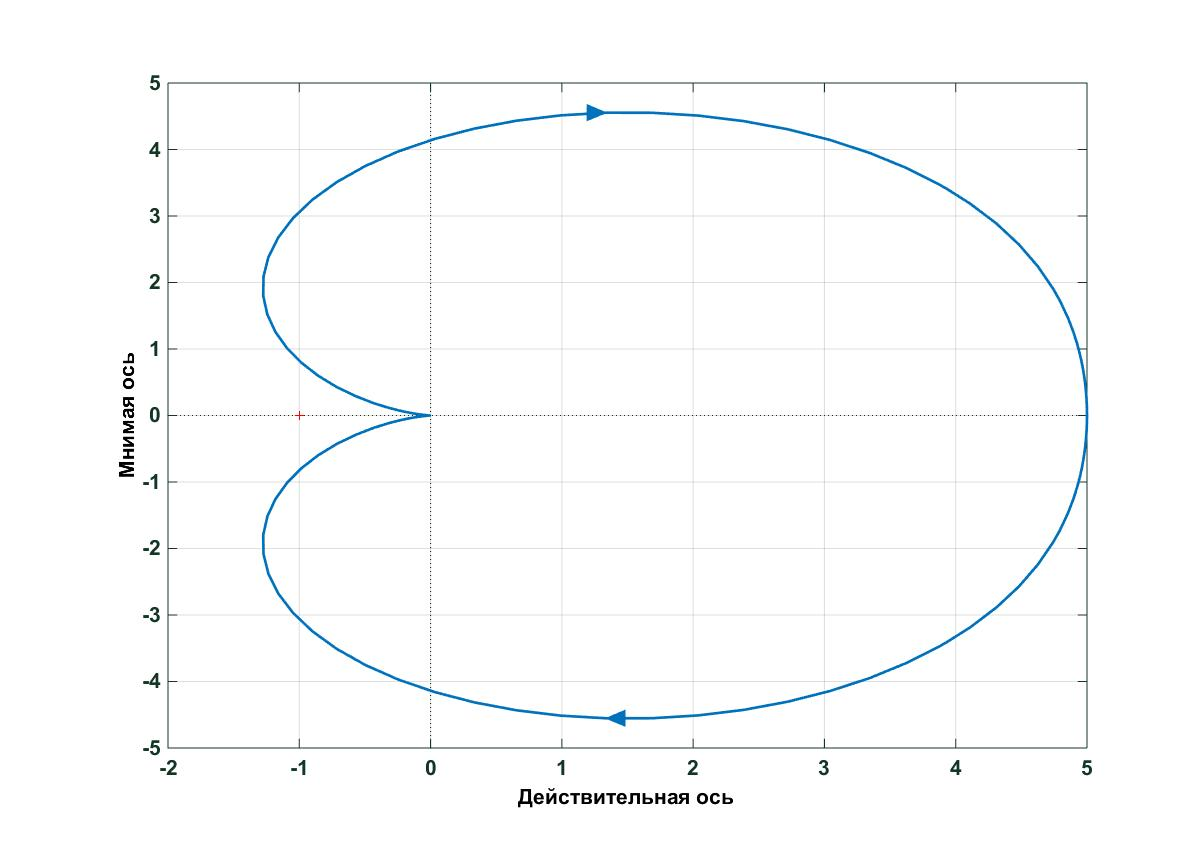
\includegraphics[width = 0.6\textheight]{data/nyquist}
	\caption{Фазовый портрет разомкнутой системы}
	\label{nyquist}
\end{figure}

На рисунке \ref{nyquist} видно, что фазовый портрет системы не огибает точку (-1; 0), другими словами, фаза системы при частоте среза меньше $-180^{\circ}.$ Следовательно, система является устойчивой по критерию Найквиста.

\newpage

\begin{center}
	\section{Анализ замкнутой системы}
\end{center}

Передаточная функция системы, замкнутой отрицательной обратной связью, будет иметь вид:
\begin{align}
\Phi(s) = \frac{s + 5}{s^3 + 6s^2 + (4+K)s + 6K}
\end{align}
где K - коэффициент обратной связи.\par
Примем К = 1, тогда передаточная функция замнутой системы принимает вид:
\begin{align}
	\Phi(s) = \frac{s + 5}{s^3 + 6s^2 + 4s + 6}
	\label{fi_my}
\end{align}

Найдем нули и полюса функции аналитически и при помощи функции Matlab - pzmap графически изобразим найденные решения на рисунке \ref{pzmap2}.\par

Из функции \ref{fi_my}  находим нули и полюса:

\begin{equation}
\begin{cases}
z_1 = 5\\	
p_1 = -5.48\\	
p_2 = -0.25 + j0.34\\	
p_3 = -0.25 - j0.34
\end{cases}
\end{equation}

\begin{figure}[h!]
	\centering
	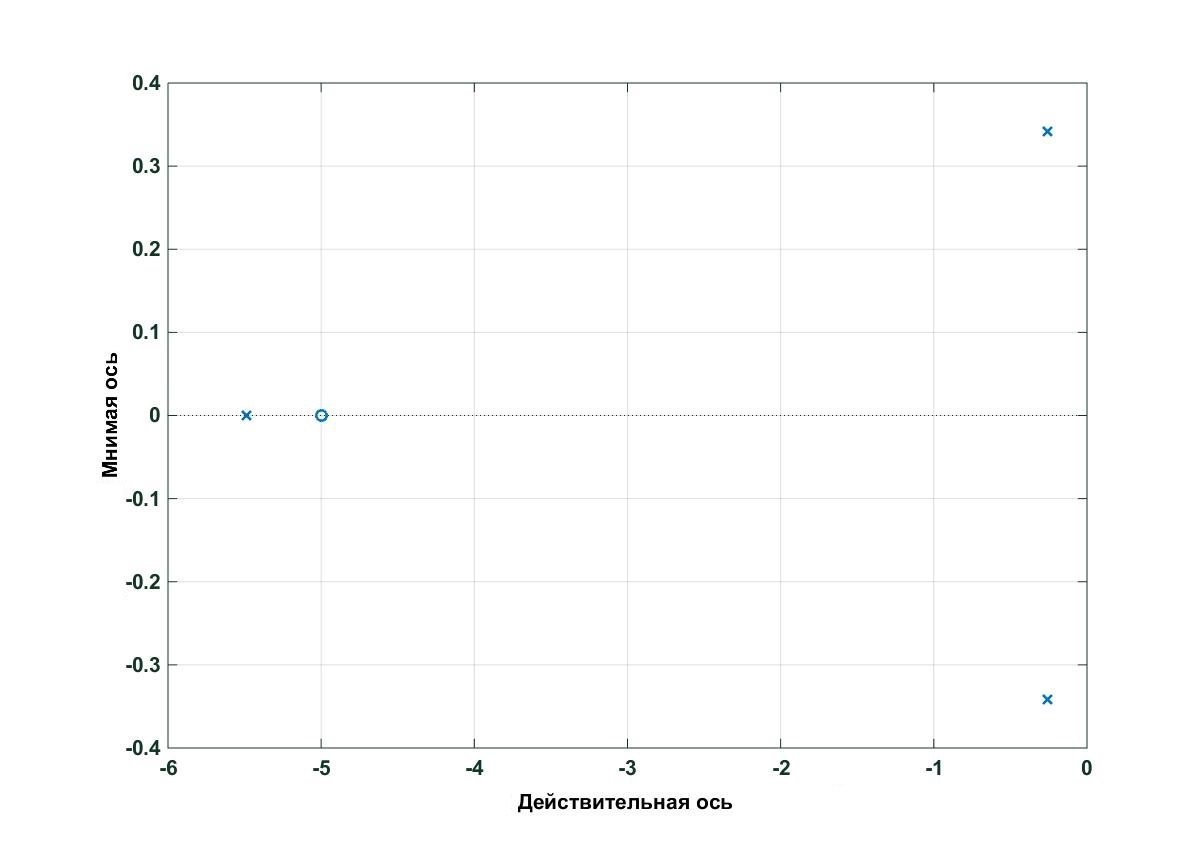
\includegraphics[width = 0.6\textheight]{data/pzmap2}
	\caption{Нули и полюса замкнутой системы}
	\label{pzmap2}
\end{figure}\par

\newpage

Воспользовавшись функциями Matlab - step и impulse построим графики переходной и весовой функции замкнутой системы. На рисунках \ref{step2} и  \ref{impulse2} результаты работы этих функций. 

\begin{figure}[h!]
	\centering
	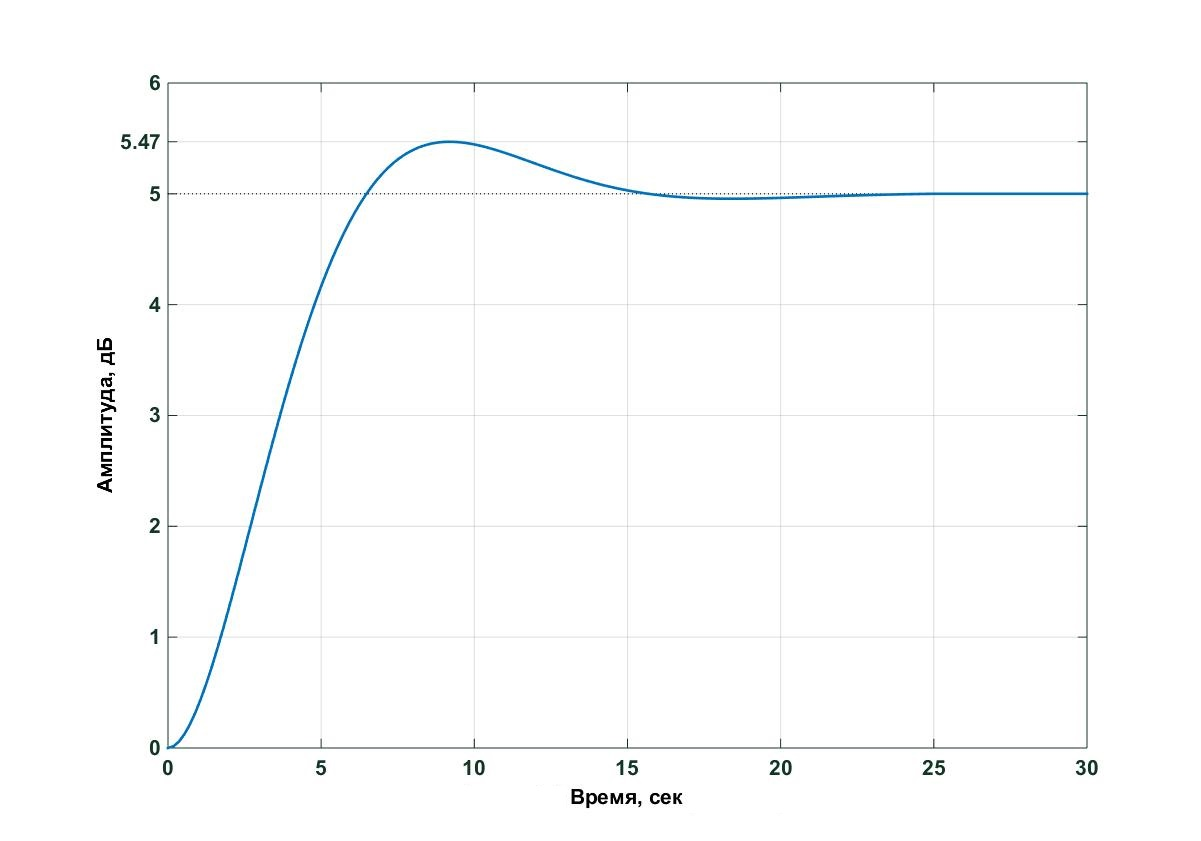
\includegraphics[width = 0.57\textheight]{data/step2}
	\caption{График переходного процесса замкнутой системы}
	\label{step2}
\end{figure}

\begin{figure}[h!]
	\centering
	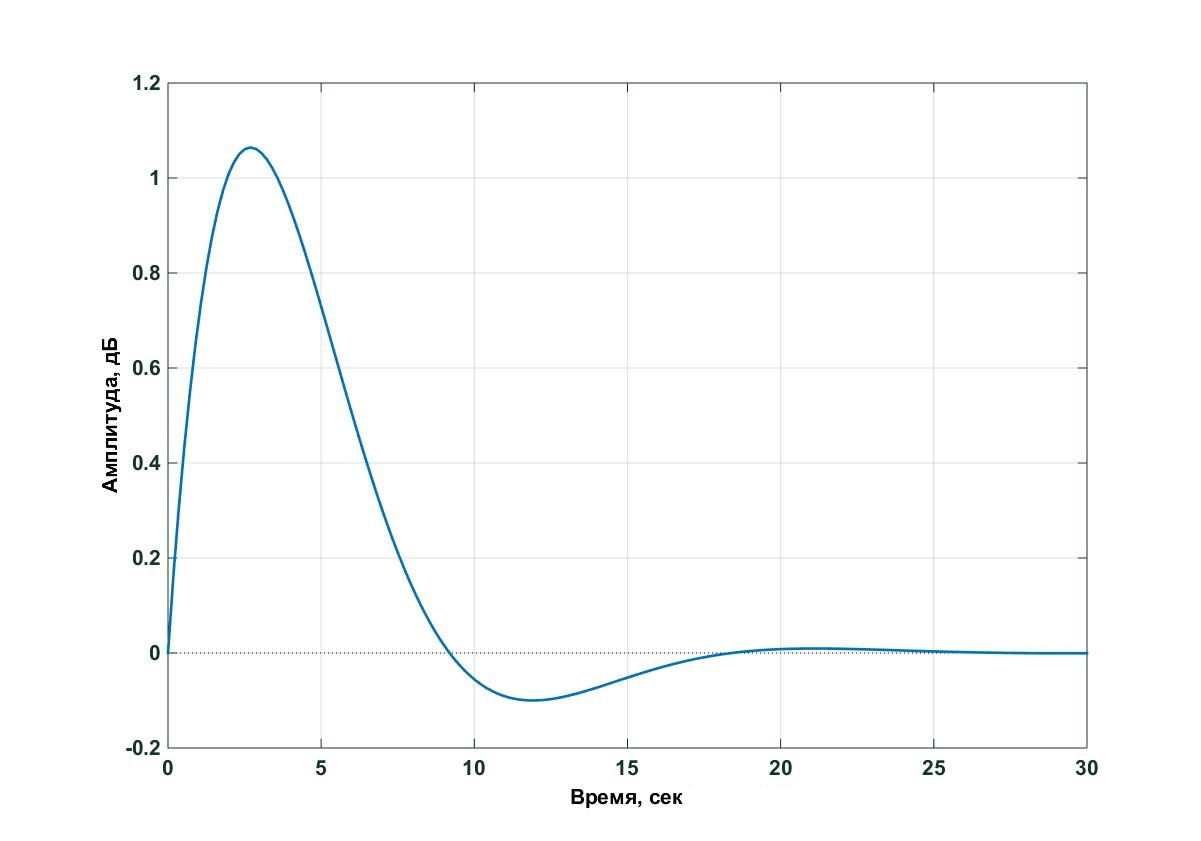
\includegraphics[width = 0.57\textheight]{data/impulse2}
	\caption{Весовая функция}
	\label{impulse2}
\end{figure}\par

\newpage

Из графика переходного процесса замкнутой системы  видно, что установившееся значение 5, время переходного процесса $t_\text{п}=25$ сек, перерегулирование $\sigma=\frac{5.47-5}{5}\cdot100\%=9.4\%$. Затухание в данной системе равно нулю.\par

Замкнутую системы можно представить в форме Вход-Состояние-Выход. Для этого воспользуемся командой $[A,B,C,D]=tf2ss(a,b)$, где $a$ числитель, $b$- знаменатель. Получим матрицы.

$A=
\begin{bmatrix}
	-6	&	-3	&	-1\\
	1	&	0	&	0\\
	0	&	1	&	0\\
 \end{bmatrix}$\\
 
$B=
\begin{bmatrix}
	1\\
	0\\
	0\\
\end{bmatrix}$\\

$C=
\begin{bmatrix}
	0	&	1	&	5
\end{bmatrix}$\\

$D=
\begin{bmatrix}
	0
\end{bmatrix}$\\

\newpage

\begin{center}
	\section*{Вывод}
\end{center}\par
В данной лабораторной работе мы исследовали разомкнутую и замкнутую систему с помощью пакета matlab control system toolbox(CST).\par
С помощью CST можно легко определить устойчивость разомкнутой системы по полюсам, отрицательная вещественная часть говорит о том, что система устойчивая. Также это подтверждается фазовым портретом, ЛАЧХ, ЛФЧХ. Из рисунка \ref{margin} видно, что запас устойчивости по амплитуде - бесконечный, это значит, что любой коэффициент обратной связи будет приводить к устойчивости системы.\par
Все это подтверждает график переходного процесса \ref{step2}, который показывает нам, что система устойчива.








\end{document} 